\section{What is your best advice when it comes to raising children?}
I realize that when I got married at 26 I adjusted to sharing life with another adult.
\begin{figure}
\centering
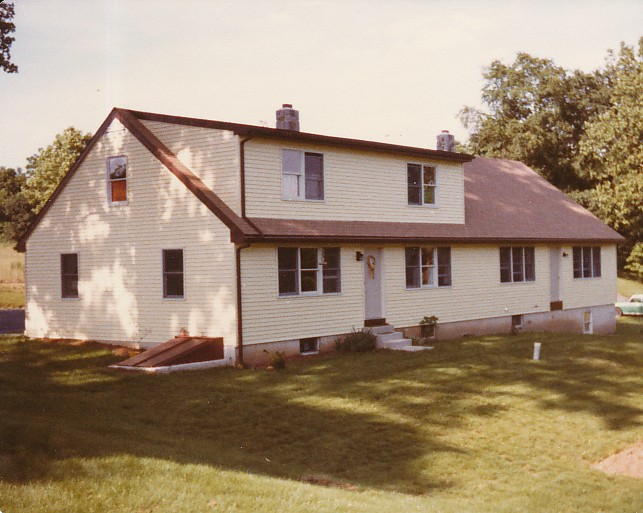
\includegraphics[width=0.9\textwidth]{our_family/18.jpg}
\caption{
Home at Blue Rock Rd
}
\end{figure}
However when our first child was born there was an even greater adjustment for me.
John and I made choices that left me the primary caregiver of the children.
Believe me that was different than being a full time teacher.
Children are needy little people and they benefit from having a parent committed to their care.
That will not always look like the system that John and I set up but it works best for all when child care is top priority for the parents.
\begin{figure}
\centering
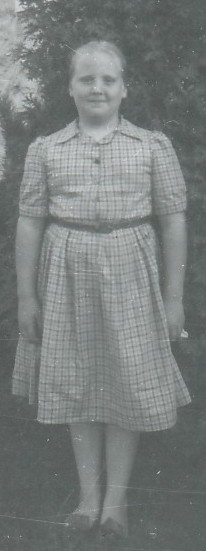
\includegraphics[width=0.9\textwidth]{our_family/20.jpg}
\caption{
Falling asleep
}
\end{figure}

Having space to be organized and the stuff you need for the child's care can help to take pressure off child care.
\begin{figure}
\centering
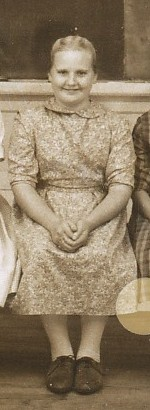
\includegraphics[width=0.9\textwidth]{our_family/21.jpg}
\caption{
Young computer programer
}
\end{figure}
I'm not suggesting the latest gadgets or fads but comfortable space for a rocking chair, crib, changing table, diaper pail, and chest of drawers for baby clothes and some kind of container for toys/books.
Simplicity can be helpful so there is not too much clutter and there is a designated space for baby care.
\begin{figure}
\centering
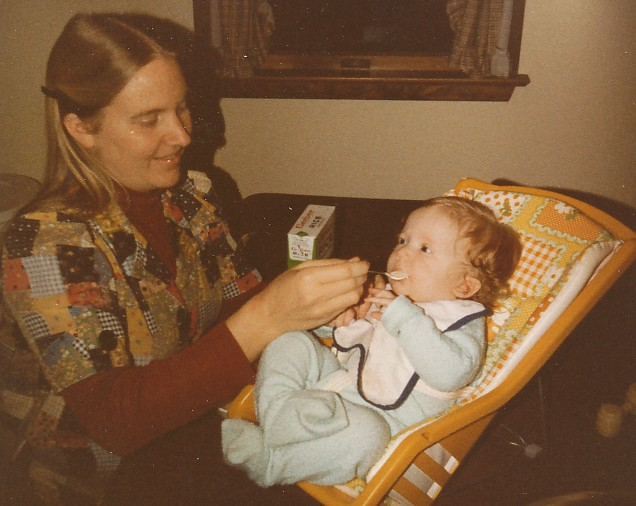
\includegraphics[width=0.9\textwidth]{our_family/22.jpg}
\caption{
Aquiring a taste for cereal
}
\end{figure}

Talk to your children.
Read to your children.

\begin{figure}
\centering
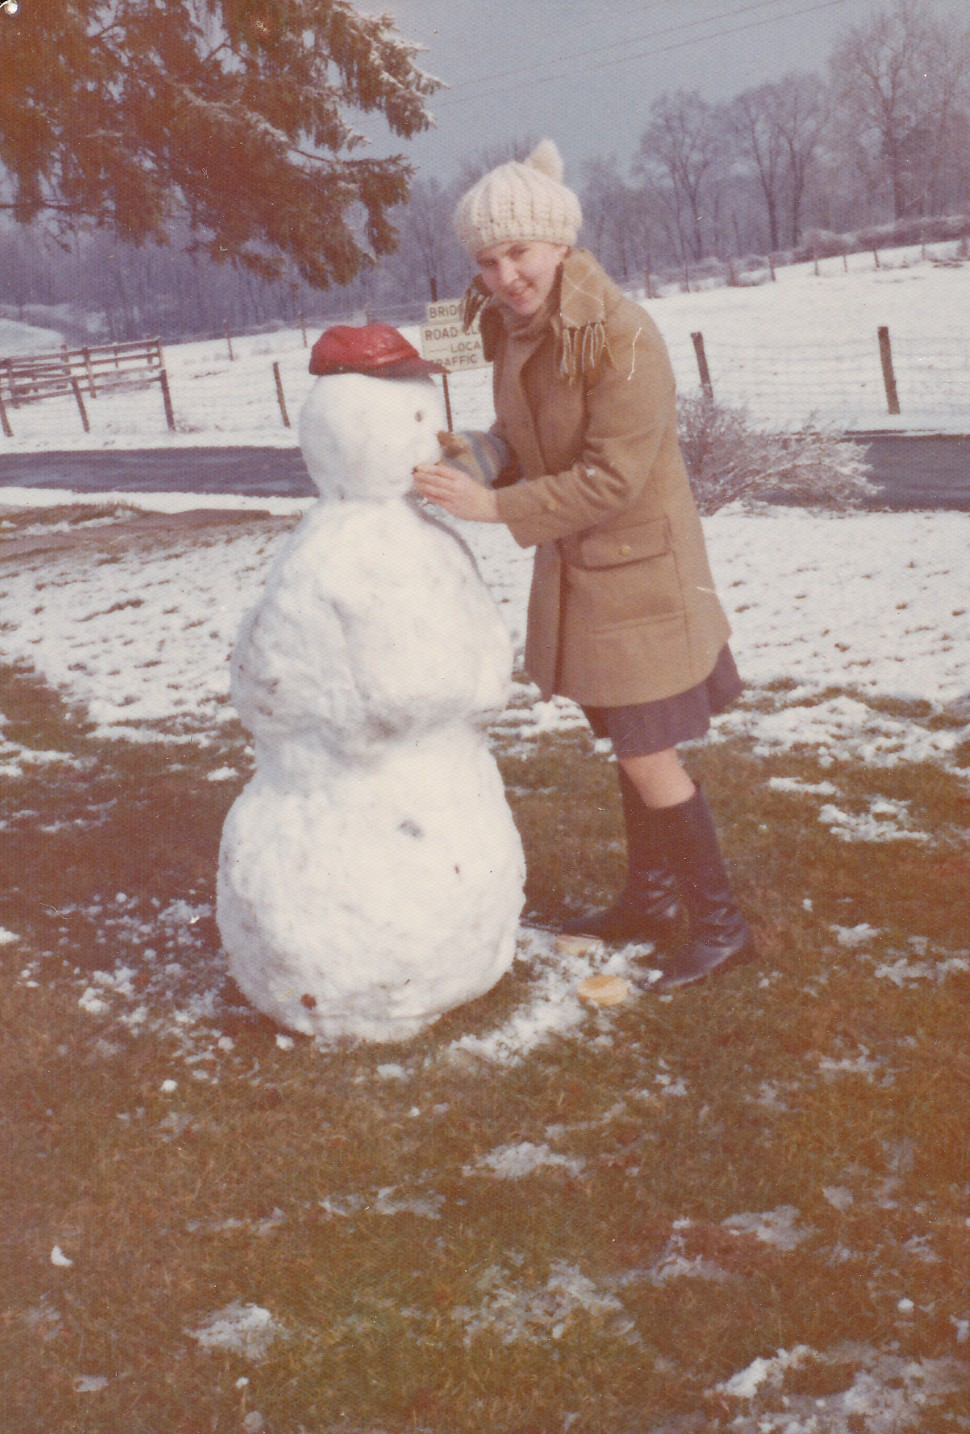
\includegraphics[width=0.9\textwidth]{our_family/24.jpg}
\caption{
Taking care of a box of tissues
}
\end{figure}
Be friends with your children.

\begin{figure}
\centering
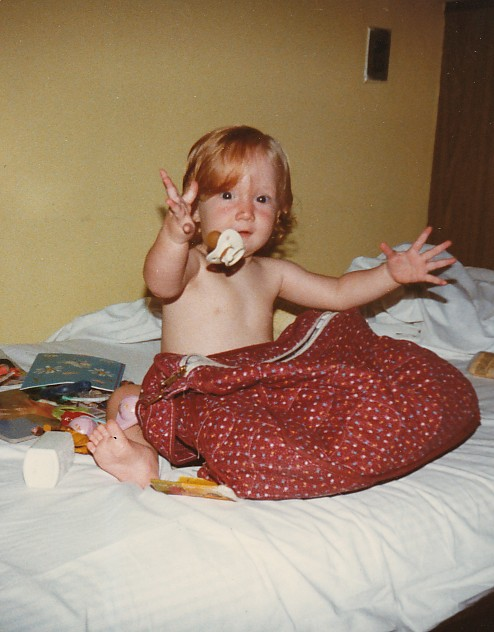
\includegraphics[width=0.9\textwidth]{our_family/25.jpg}
\caption{
No need for a pacifier. 
}
\end{figure}
Give time to your children.

\begin{figure}
\centering
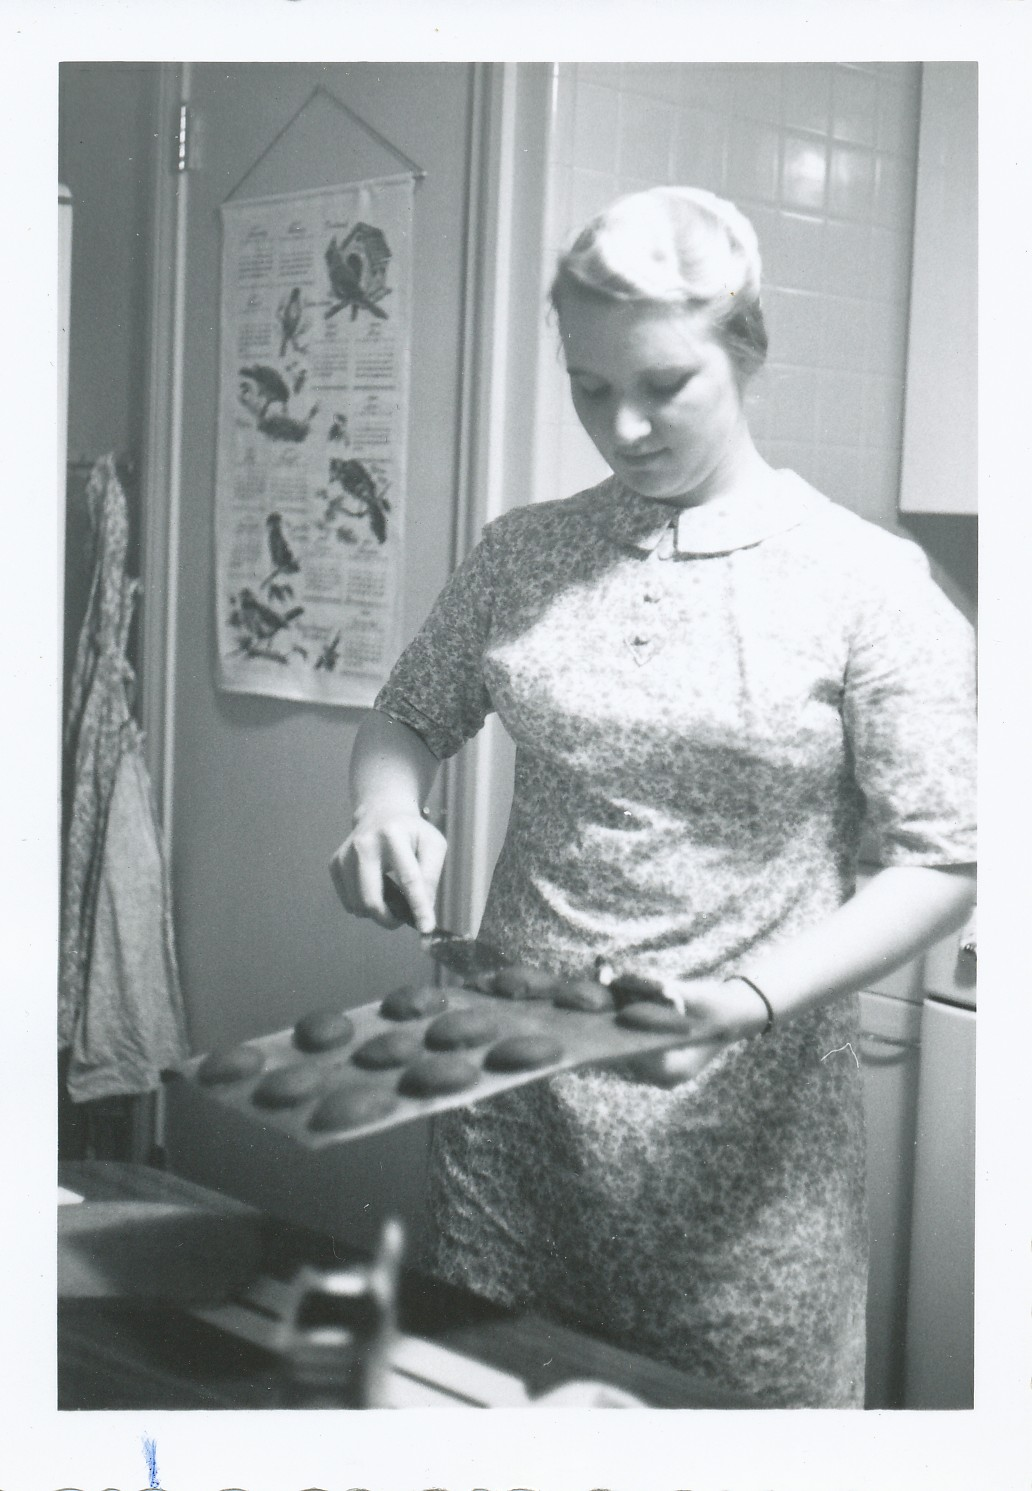
\includegraphics[width=0.9\textwidth]{our_family/23.jpg}
\caption{
Burping
}
\end{figure}

They should know that they are a priority of their parents.

\begin{figure}
\centering
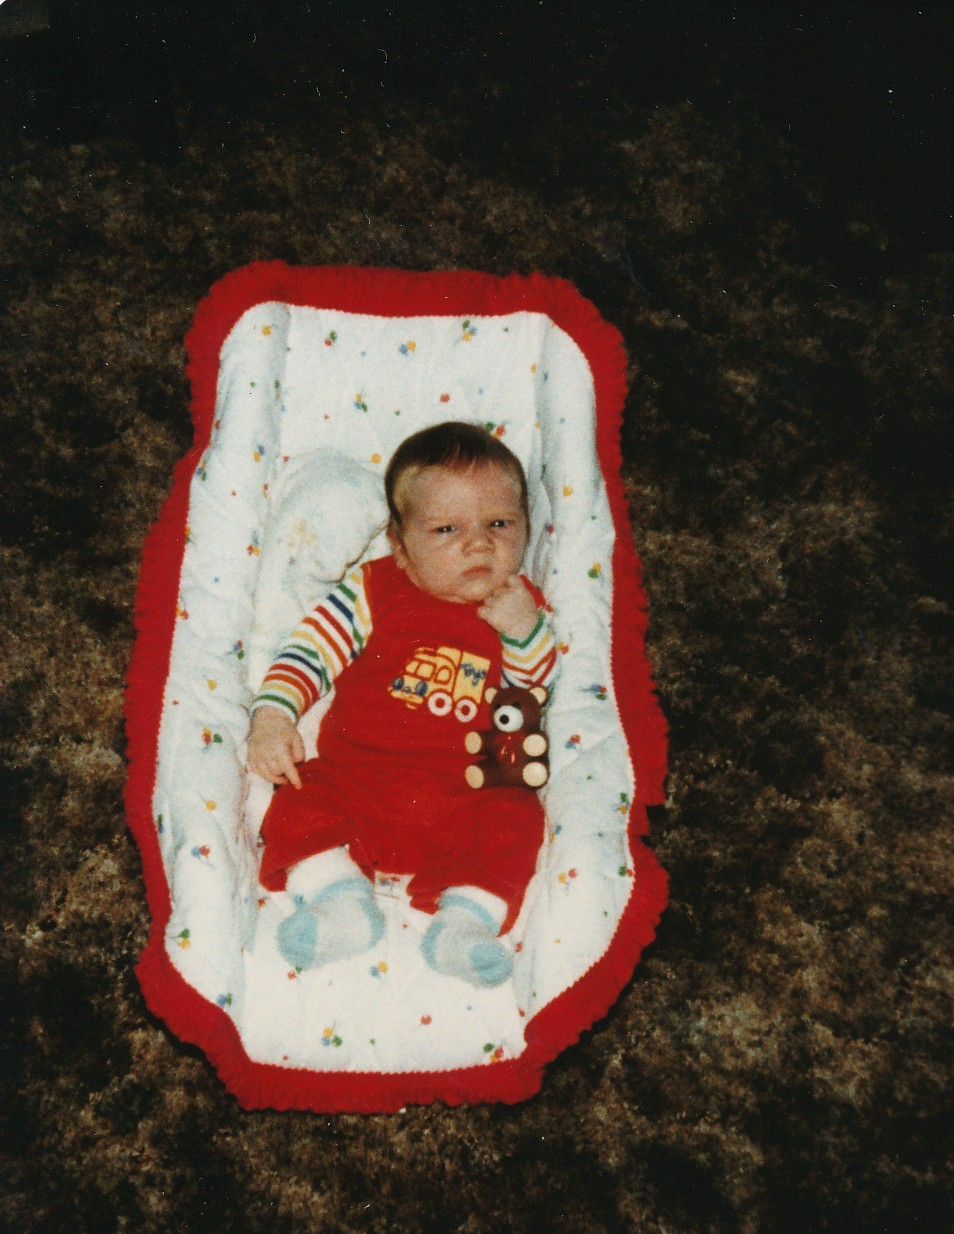
\includegraphics[width=0.9\textwidth]{our_family/26.jpg}
\caption{
Pondering great thoughts
}
\end{figure}

\begin{figure}
\centering
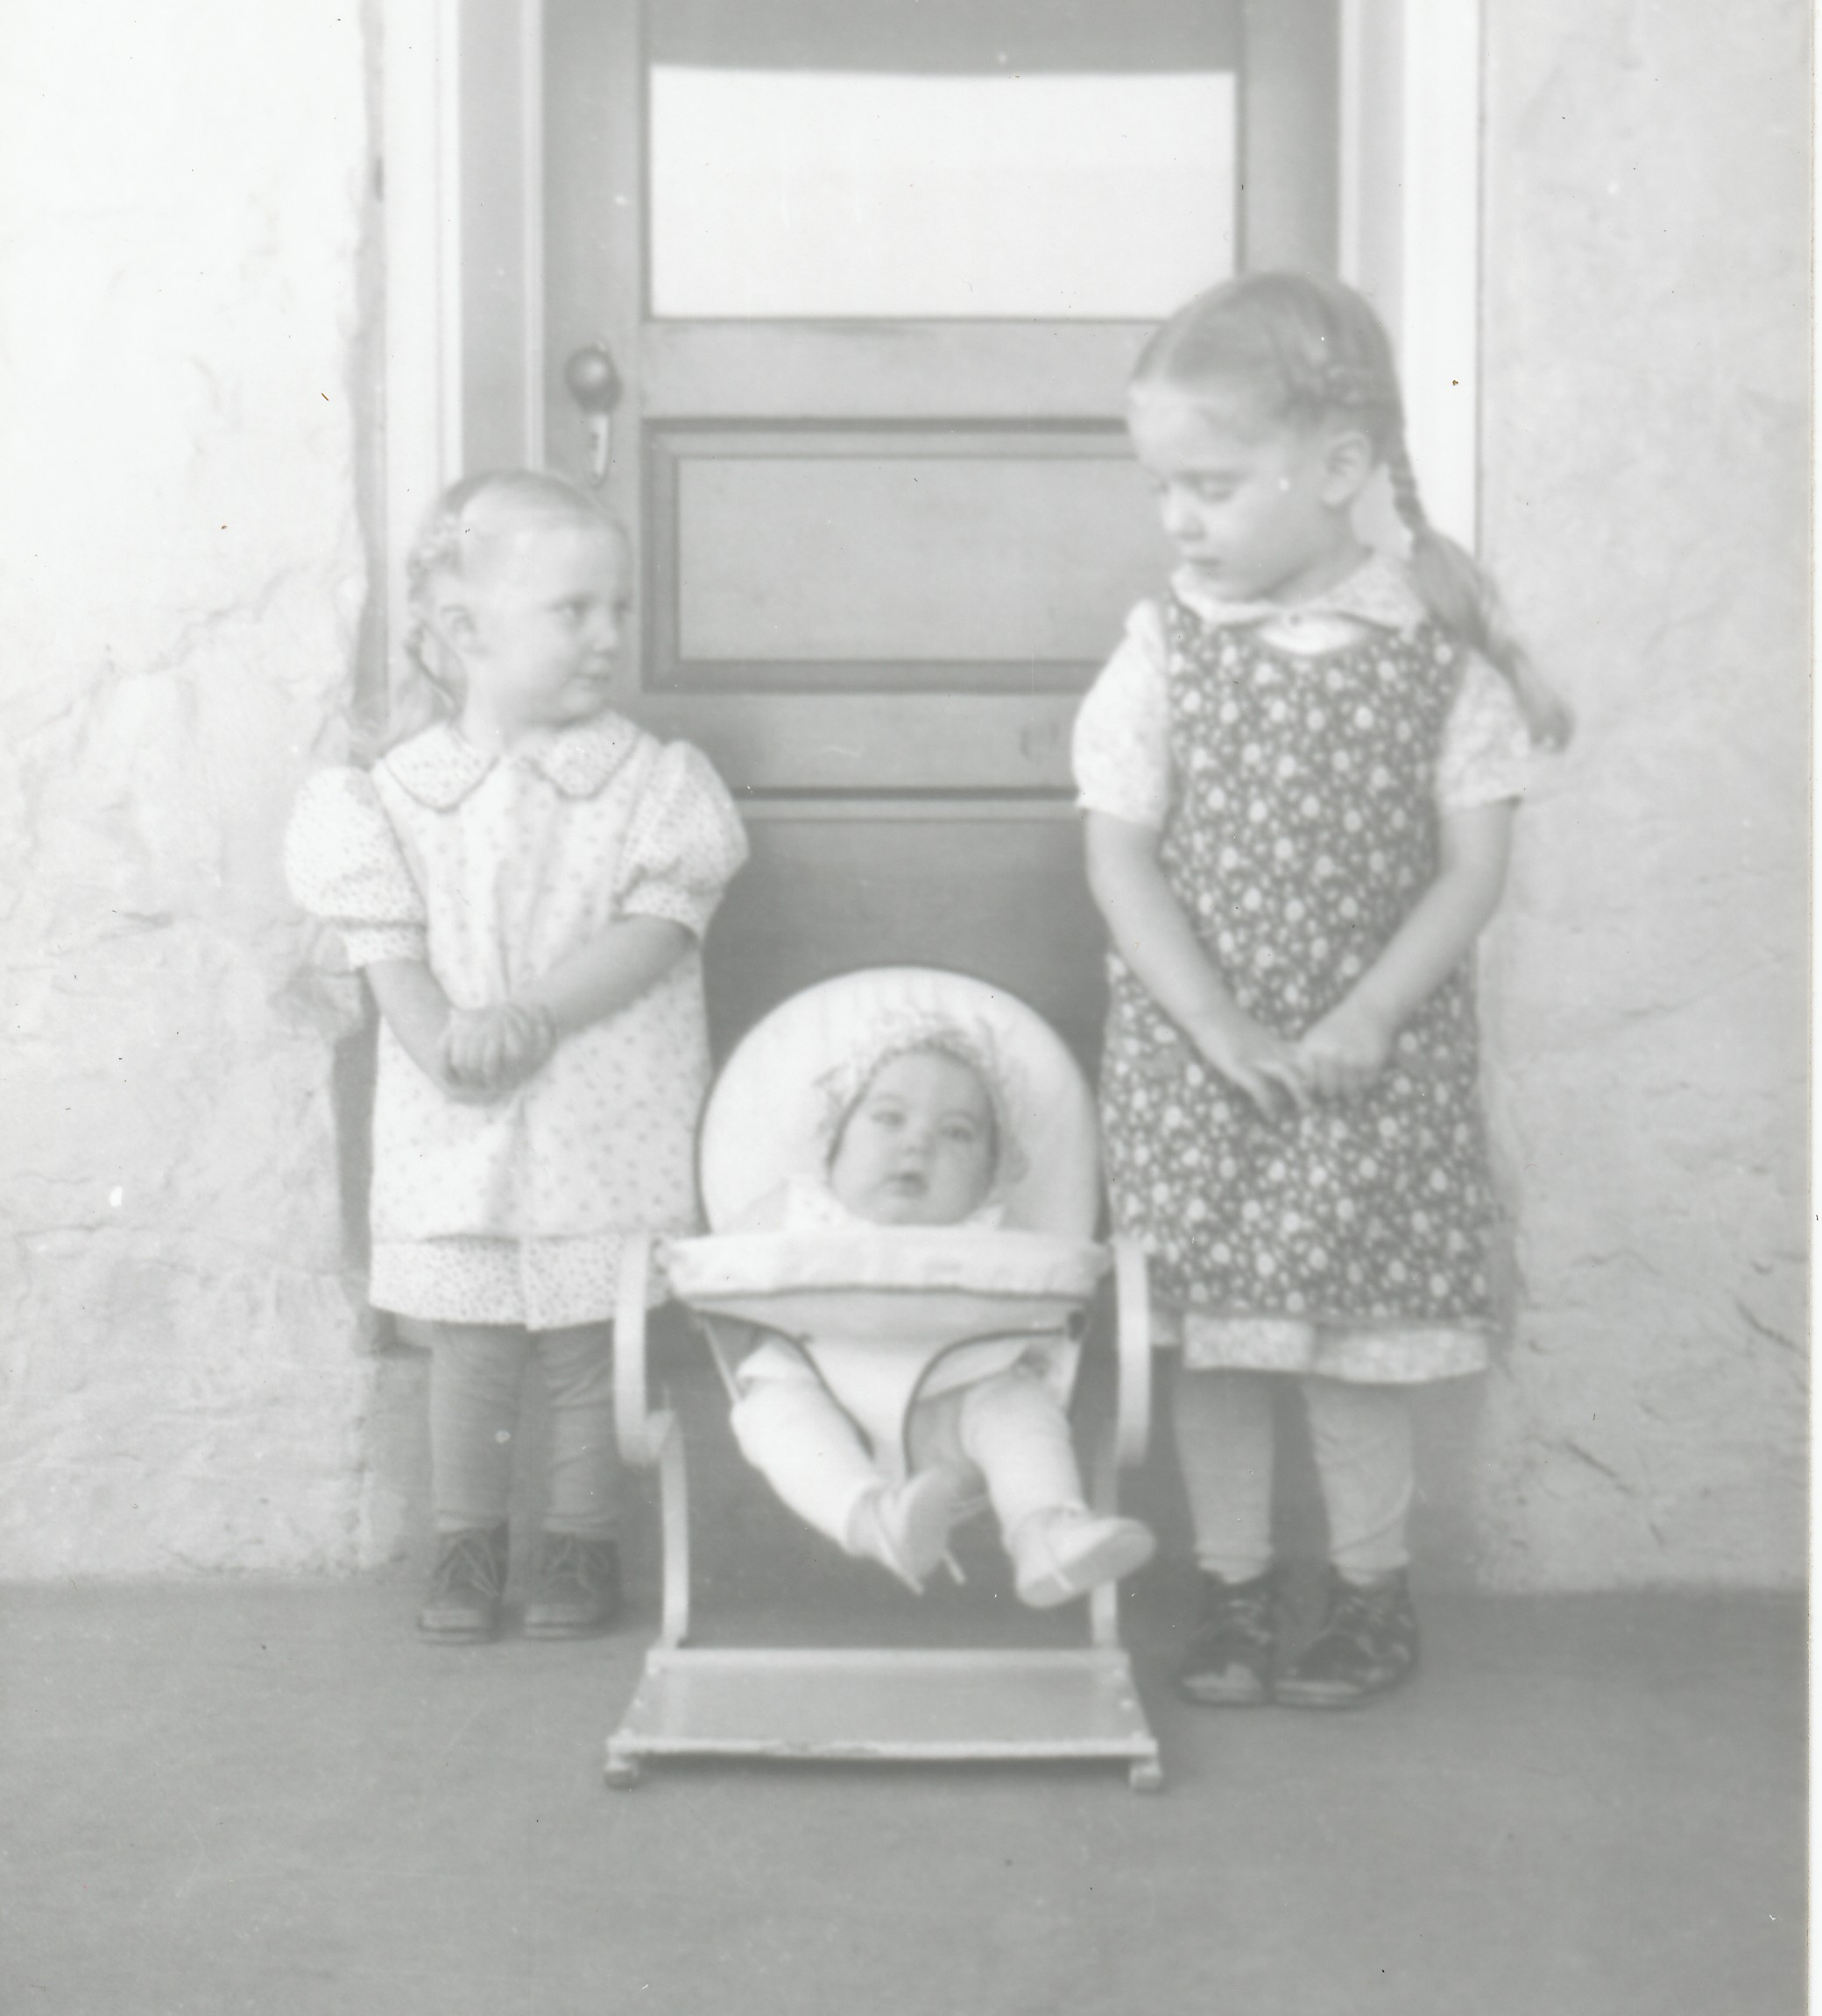
\includegraphics[width=0.9\textwidth]{our_family/27.jpg}
\caption{
A bucket full of Jonathan 
}
\end{figure}

Having said that I made the difficult decision with John's support to come to study at AMBS when my children were still in elementary school.
This was not an easy move for my children or for any of us for that matter.
In the long run it may have saved my life and given all of us some fresh air and new space to explore.
To some I'm guessing it looked like a selfish decision on my part.

From Abby - This is lovely Mom! Thanks for all the good advice and I should say that while I don't know how I responded to it at the time, I have often pointed to your decision to go to AMBS as a critical one for me in realizing that the needs of mothers and wives are just as important as those of fathers and husbands.
I am very grateful that you and Dad gave me and my brothers that example and many others of how a more equal partnership can be formed and nourished through the years.





